\section{Results}~\label{sec:results}
In this section, we present our comparison results and our insights for designing better grouping tools.

\subsection{Comparison based on Grouping Criteria}
RQ1: Why do we group crash dumps?
\begin{enumerate}
\item Besides grouped based on the same root cause, crash dumps can also be correlated if the patch to one crash is the cause for another crash.
\item Developers also group crash dumps if they can be conveniently fixed together, for example, by a same developer.
\item Diagnosing a group of crash dumps can be beneficial: first, a group of symptoms help determine general manifestation of a bug; second, a group of similar call stacks potentially enable automatic bug localizations. 
\end{enumerate}

\begin{table}[!htb]
\centering
\caption{Grouping Criteria for m-Groups\label{tab:goal}}
\resizebox{\columnwidth}{!}{
\begin{tabular}{|l||l|l|}\hline
Grouping Criteria&Goals\\\hline\hline
\multirow{4}{*}{Same Root Cause}&Fix one to fix all in the group\\\cline{2-2}
&Determine if a given new crash is fixed\\\cline{2-2}
&Localize bugs via comparing similar stacks\\\cline{2-2}
&Learn bug manifestation to prioritize them\\\hline\hline
\multirow{2}{*}{Related Root Cause}&Localize root causes if fix to previous\\
&crashes is the cause for the current crash\\\hline\hline
\multirow{2}{*}{Who Fix the Bug}&Find experts who can fix a group of bugs\\
&from the same code region or of same types\\\hline
\end{tabular}
}
\end{table}

%\begin{figure}
%\begin{minipage}[b]{\textwidth}
%\centering
%\includegraphics[width = \columnwidth, angle = 0]{group.ps}
%\end{minipage}
%\caption{Fault Localization Based On Call Stacks~\label{fig:group}}
%\end{figure}

For automatic approaches that compare call stack similarity for grouping crash dumps, the implied grouping criterion is that the crash dumps in a group should share the root cause. However, we find that the grouping criteria applied in manual diagnosis are more diverse and flexible. 

In Table~\ref{tab:goal}, we summarize our discoveries. Similar to automatic approaches, in many cases, developers correlate crash dumps if they believe these crashes are originated from the same bug in the code. In another word, if we introduce a fix based on any crash in the group, we can fix all the crash dumps grouped, and if a new crash dump is determined to belong to the group, we do not need to further diagnose it.

Interestingly, although the goal of grouping crash dumps is to avoid repeatedly diagnosing crash dumps caused by the same root cause, developers sometimes still compare multiple crash dumps in the same group for determining the types and locations of a bug. It indicates that a group of crash dumps can be more informative than individual crash dumps in helping diagnose failures. For example, a same bug may cause completely different symptoms, and we find a case where developers prioritize a group of crash dumps because one of the crashes have the serve symptom related to a security attack. 

As shown in the table, developers also correlate crash dumps if the root causes that lead to the crashes have a temporal or locality relationship. In our study, we find cases where one crash is caused by an incomplete/incorrect fix to the other crashes. Developers believe that correlating these crashes can help quickly identify the cause and the fix for the newly generated crashes.

In addition, developers group crash dumps using the criterion of who can fix them. Here, the components where the crashes occur, together with the bug types, are used to determine the groups. The goal is to better distribute the debugging tasks to people who are most familiar with the code and the bug types.

\subsection{Comparison based on Grouping Information}

RQ2: What information shall we use to group crashes?
\begin{enumerate}
\item Call stacks, build information and reproduce steps are the three main sources for developers to group crashes.
\item Developers frequently correlate multiple sources of information for determining the groups. For example, developers once linked call stacks and reproduce steps by comparing call stacks in crash dumps with the call stack in a non-crash thread.
\item Developers correlate crash dumps across applications to determine if the root cause is located in the shared libraries or plugins.
\item Different versions of programs can contain the same piece of problematic code, and thus we should enable the grouping across different versions of the code.
\end{enumerate}


\begin{figure*}
%\begin{minipage}[b]{\textwidth}
%\subfigure[Same Signature, Different Causes]{
\subfigure[List of Information Source]{
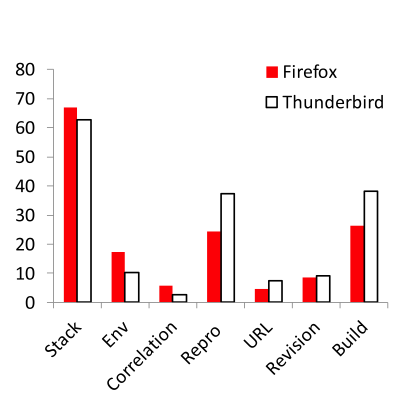
\includegraphics[width = 6.6 cm, angle = 0]{Info1.ps}
~\label{fig:ind}
}
\subfigure[Linking Multiple Sources]{
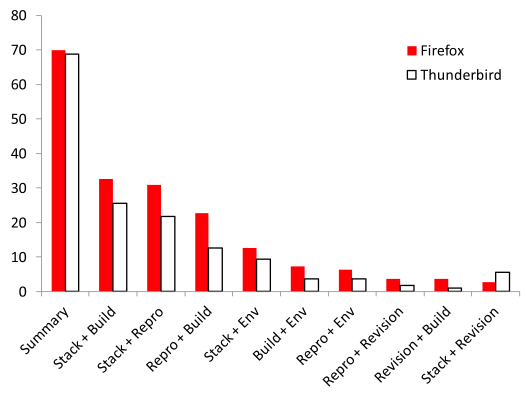
\includegraphics[width = 9.0 cm, angle = 0]{Info2.ps}
~\label{fig:multi}
}
%\end{minipage}
\caption{Information Used for Manually Grouping Crash Dumps~\label{fig:stack}}
\end{figure*}

Mozilla Crash Reporter automatically groups crash dumps by matching 1) the version of software where the crash dumps are originated; and 2) the function call on the top of the call stack at the crash, called {\it signature}. On the contrarily, developers use a variety of information. No systematic way is applied to choose which source of information should be used for determining a particular group of crash dumps.

We studied a total of 40 m-groups from Firefox and Thunderbird. We find that developers generally apply three types of information for grouping crash dumps: 1) white-box information, i.e., crash symptoms related to code including call stacks and their signatures, 2) black-box testing information, e.g. steps on triggering the bug, and 3) information related to software versions, such as build time and revision histories. 

We summarize our analysis results in Figure~\ref{fig:stack}. On the left, we rank a list of information source developers frequently use in determining crash dump groups, and on the right we show the correlation of these sources applied in manual diagnosis. The $y$-axis presents the percentage of crash dumps that are grouped using the specific source(s) of information.

In Figure~\ref{fig:ind}, along the $x$-axis, {\it Stack} represents call stacks. {\it Env} indicates the plugins and libraries involved in the crash. {\it Correlation}, used by Mozilla Crash Reporter, specifies how often a signature and a .dll component are simultaneously witnessed in a crash. For example, given a set of call stacks, we count that a certain signature occurs 10 times, and among the 5 times, a specific .dll also occurs; in this case, the correlation ratio between the signature and the component is 50\%. {\it Repro} and {\it URL} indicate two relevant types of testing information. {\it Repro} represents the steps taken to reproduce the bug and {\it URL} refers to a list of URL visited before an application crashes. {\it Revision} is a list of changes made to the application shortly before a crash. Finally, {\it Build} gives the date and time to indicate when the application is built and installed, as well as the version of operating system where the application runs.

Figure~\ref{fig:ind} shows that call stack, build information and reproduce steps are the three most frequently used sources. For Firefox, 67\% of the crash dumps were grouped using call stacks, 26.4\% applied build information and 24.5\% were determined using reproduce steps. Similarly, for Thunderbird, 62.7\% used call stacks,  38.2\% used the build information and 37.3\% applied reproduce steps. The secondary important source is {\it Revision}, based on which, 8.5\% of the Firefox crash dumps and 9.1\% of the Thunderbird crash dumps are grouped. By inspecting m-groups determined using {\it Revision} information, we find that when crashes occur shortly after a new release of an application, plugin or operating system, developers give the priority to consider whether the crash dumps can be caused by the same bug in the new code and thus can be grouped together. Sometimes, the developers suspect that the crash dumps are caused by bugs in a certain plugin or operating system, and thus they correlate crash dumps from different applications running with the same plugin or operating system.

% developers would determine if a particular type of crash dumps only occur after new releases of applications, plugins or even operating systems. Consider the number of bugs in new code may be small, the crash dumps are likely to be caused by the same bug in the new code and thus can be grouped together. If developers suspect the crash dumps are related to plugin or OS, they link crash dumps from multiple applications.

 %It is useful in determining if, and what recent alterations may have caused the crash. If a previous patch would have fixed or caused the issue. This is the same as looking to see if a previous build of the application could have caused the issue, or if it is used to find correlations between bugs.  If the occurrence of the crash is correlated to a major release with operating systems such as Windows patches, crash dumps occurred at the similar time, will be attributed to as likely due to a bug in new release code. Sometimes they will group crash dumps from multiple applications that run in the same environments.

In Figure~\ref{fig:multi}, we show that developers often make decisions by coordinating multiple sources of information. The leftest bars in the figure indicate that 70\% of the crash dumps from Firefox and 68.8\% from Thunderbird are grouped by using more than one source of information. Consistent with Figure~\ref{fig:ind}, developers most frequently link call stacks, build information and reproduce steps to determine the groups. As shown in Figure~\ref{fig:multi}, the top three combined-sources include 1) call stack with build information, 2) call stack with reproduce steps and 3) reproduce steps with build information. Correlating Figure~\ref{fig:ind} and~\ref{fig:multi}, we can obtain interesting findings. For example, we can derive that 67\% of the Firefox crash dumps are grouped using call stacks, among which, about a half are used with the reproduce steps and a half are used with build information. The three of the sources might be used together in some cases. 

Our inspection in m-groups shows that developers often use build information as the first step to reduce the scope of the grouping. However, grouping crash dumps of the same version sometimes is not ideal because different versions of a program may contain the same problematic code and any crash dumps caused by this code should be grouped. 

We also discover that coordinating call stacks and reproduce steps can be challenging. We find a case where developers compare a crash dump with call stacks in non-crash threads to determine what steps in testing can produce a specific sequence of calls in the call stacks.

%The build information helps determine which version of code the crash is originated. The rationale is that crash dumps in a group 1) could origniate from different versions of code, but all of which should contain a same bug 2) manifest similarity in call stacks and/or 3) crash dumps can be reproduced following the similar steps. Automatic approach groups stack only based on the same version of code can miss related crash dumps. We need to find a way to correlate call stacks and reproduce steps.

\subsection{Comparison based on Imprecision}

RQ3: when do we group unrelated crash dumps and when do we fail to find the relevant crash dumps? 

\begin{enumerate}
\item Imprecision in m-groups is caused by developers' mistakes, and sometimes, a simple mistake can take months to recover.
\item Grouping purely based on the similarity of call stacks is insufficient; especially some applications can generate very dissimilar call stacks at the crash.
\end{enumerate}

We first show our results on imprecision in m-groups. In Table~\ref{tab:mistake}, we list the four examples confirmed as developers' mistakes. Under {\it Bug ID}, we list the identifications of the Bugzilla entries where the mistakes are found. Under {\it Developers' Mistakes}, we give the descriptions of the mistakes. Under {\it Time}, we show the time period from when the mistake is firstly introduced to the Bugzilla post to when the developers confirm the problems. In the first two cases, developers misread the call stacks and mismatched the code. In the third case, developers only used signatures, the approach implemented in Mozilla Crash Reporter, rather than performed a more depth analysis to determine the group. In the fourth case, developers made a wrong judgment and believed the crash is a regression of a previous a bug. The results show that these mistakes can be difficult to discover, and the time that takes to find the problems is not always proportional to how complicated a mistake is about. The implication of this result is that we need to develop automatic tools to help avoid these simple but expensive mistakes from developers.
\begin{table}[!htb]
\centering
\caption{Imprecision in m-Groups: Example Mistakes\label{tab:mistake}}
\resizebox{\columnwidth}{!}{
\begin{tabular}{|c||l|l|}\hline
Bug ID&Developers' Mistakes&Time\\\hline\hline
716232&Mismatch call stacks&4.6 hours\\\hline
695505&Inspect wrong version of code&3.0 months\\\hline
524921&Match signature only&2.7 days \\\hline
703133&Incorrectly link to a patch& 4.7 days\\\hline
\end{tabular}
}
\end{table}

\begin{table}[!htb]
\centering
\caption{Imprecision in a-Groups\label{tab:agroup}}
\resizebox{\columnwidth}{!}{
\begin{tabular}{|c||c|c|c|}\hline
Total&Corrupted Stack&Group Unrelated& Fail to Group Related\\\hline\hline
100&4&2&4\\\hline
\end{tabular}
}

\end{table}

In Table~\ref{tab:agroup}, we present the set of data that demonstrate the imprecision in a-groups. Our approach is to inspect the Bugzilla entries that document the manual diagnosis for the a-groups and find imprecision in a-groups confirmed by developers. Under {\it Total}, we show that we studied the Bugzilla entries related to a total of 100 a-groups in our dataset. Under {\it Corrupted Stack}, {\it Group Unrelated}, and {\it Fail to Group Related}, we list the number of instances for the three types of imprecision: 1) call stacks are corrupted at the crash and thus the signature returned is no longer the top function where the actual failure occurs; 2) crash dumps grouped in an a-group are actually irrelevant; and 3) crash dumps of the same/related root causes are not grouped in the same a-group. 

In our study, we find that all of the three types of imprecision exist in a-groups. The actual instances may even be higher than the ones listed in the table, as developers may only discover a small portion of such problems. In the following, we present two examples discovered during inspecting these mistakes. The examples indicate that it is neither sound nor complete to group crash dumps only based on the equivelance of the signatures or the similarity of the call stacks.

In Figure~\ref{fig:group2}, the two crash dumps are generated from the same cause in the same version of the program. However, because the crashes are triggered in different versions of Windows, the crash dumps contain different signatures (see the first row in the table) and thus were not grouped by Mozilla Crash Reporter.

\begin{figure}
\centering
\resizebox{\columnwidth}{!}{
\begin{tabular}{|l|l||c|}\hline
Call Stack 1 & Call Stack 2 & Match\\\hline\hline
\multirow{2}{*}{\_SEH\_prolog}& InternalCallWinProc &\multirow{2}{*}{$\times$} \\\cline{2-2}
&UserCallWinProcCheckWow &  	\\\hline
CallWindowProcAorW & CallWindowProcAorW & $\checkmark$\\\hline
CallWindowProcW  & CallWindowProcW & $\checkmark$\\\hline
mozilla::plugins::PluginInstance&mozilla::plugins::PluginInstance&\multirow{2}{*}{$\checkmark$}\\
Child::PluginWindowProc & Child::PluginWindowProc &  \\\hline
InternalCallWinProc &InternalCallWinProc  & $\checkmark$ \\\hline
%js::mjit::Compiler::checkAnalysis &js::mjit::Compiler::checkAnalysis &js::analyze::ScriptAnalysis::analyzeTypes \\\hline
\end{tabular}
}
\caption{Same Cause, under Different Versions of OS, result in Different Signatures~\label{fig:group2}}
\end{figure}

In Figure~\ref{fig:stack2}, we show that by only comparing the similarity between call stacks, we can fail to distinguish a legitimate and illegal correlation between the call stacks. On the left in Figure~\ref{fig:stack2}, the two call stacks have the same signatures and 19 out of 26 calls in the first call stack have appeared in the second call stack. On the right of the figure, the two call stacks also contain the same signatures; however, only 10 out of 30 calls in the first call stack have appeared in the second. In fact, developers confirm that the first pair have irrelevant root causes, while the second pair should be correlated.  Any techniques using call stack similarity for grouping crash dumps could fail to correctly group the call stacks in the two cases.

\begin{figure*}
\resizebox{\textwidth}{!}{
\subfigure{
\begin{tabular}{|l|l||c|}\hline
\multicolumn{3}{|c|}{Match 19/26, Different Causes }\\\hline\hline
js\_DestroyScriptsToGC&js\_DestroyScriptsToGC&$\checkmark$\\\hline
thread\_purger&PurgeThreadData&$\times$\\\hline
...&...&...\\\hline
XRE\_main&XRE\_main&$\checkmark$\\\hline
main&CloseHandle&$\checkmark$\\\hline
\end{tabular}
}
\subfigure{
\begin{tabular}{|l|l||c|}\hline
\multicolumn{3}{|c|}{Match 10/30, Same Causes}\\\hline\hline
JSObject::nativeSearch & JSObject::nativeSearch&$\checkmark$\\\hline
js::LookupPropertyWithFlags & js\_LookupProperty& $\times$ 	\\\hline
...&...&...\\\hline
nsINode::DispatchEvent &@0xffffff81&$\times$\\\hline	
nsContentUtils::DispatchTrustedEvent&nsArrayCC::Release&$\times$\\\hline
\end{tabular}
}
}
~\label{tab:stack}
\caption{Call Stack Similarity Fail to Distinguish Legitimate and Illegal Groups~\label{fig:stack2}}
\end{figure*}

\subsection{Comparison based on Call Stack Characteristics}

RQ4: Does automatic and manual approaches group a similar set of crash dumps?

\begin{enumerate}
\item Automatic approach is scalable in that it can correlate hundreds of crash dumps and group stacks with thousands of calls; however, the developers' knowledge about the code is more effective in grouping crash dumps in small applications.
\item Call stacks in an m-group are more dissimilar from each other than ones in an a-group, suggesting manual diagnosis can group more varieties of crash dumps that are not able to be grouped by automatic approaches.
\item Call stacks correlated in a-groups and m-groups are more similar among each other than the ones randomly grouped, suggesting call stack similarity can be an indicator of  sharing a same or related cause and can be used as one factor to determine groups of crash dumps.

\end{enumerate}
\begin{table*}
\centering
\caption{Sizes of Crash Dump Groups and Call Stacks in m-Group and a-Group\label{tab:size}}
\resizebox{\textwidth}{!}{
\begin{tabular}{|l||c|c|c|c|c|c||c|c|c|c|c|c|c|}\hline

\multirow{2}{*}{Program} & \multicolumn{6}{|c||}{a-Groups} & \multicolumn{6}{|c|}{m-Groups} \\\cline{2-13}

&G$_{max}$&G$_{min}$&G$_{ave}$&L$_{max}$&L$_{min}$&L$_{ave}$&G$_{max}$&G$_{min}$&G$_{ave}$& L$_{max}$&L$_{min}$&L$_{ave}$ \\ \hline\hline

Firefox 14.0a1&8645&13&61.5&1854&46&1925.5&39&3&11.7&1035&61&412.2\\ \hline
Thunderbird 10.0&355&2&10.5&8864&6&333.6&33&3&11.9&1024&93&376.1\\ \hline
Fennec 2.1.2&2233&1&8.6&13832&2&415.5&24&3&7.8&1456&46&306.2\\ \hline
Fennec Android 13.0a1&993&2&16.6&12697&4&659.2&24&3&9.5&1456&82&360.2\\ \hline
SeaMonkey 2.7.2&15&1&2.0&686&2&76.5&16&3&7.4&596&6&237.9\\ \hline

\end{tabular}
}
\end{table*}

In this section, we present our results on comparing sizes of grouped crash dumps and the similarity of call stacks in the groups. From the characteristics of grouped call stacks, we aim to find implications on capabilities of the two approaches in grouping crash dumps.

In Table~\ref{tab:size}, under {\it G$_{max}$},  {\it G$_{min}$} and {\it G$_{ave}$}, we report the maximum, minimum and average numbers of call stacks in the a-groups and m-groups under study. Under {\it L$_{max}$}, {\it L$_{min}$} and {\it L$_{ave}$}, we show the maximum, minimum and average lengths of the call stacks that are grouped. Comparing the data under {\it G$_{max}$} and {\it G$_{ave}$}, as well as {\it L$_{max}$} and {\it L$_{ave}$} for the a-groups and m-groups, we find that automatic approach is more scalable; it groups more crash dumps and the crash dumps handled are generally much larger.

An exception is the smallest program {\it SeaMonkey}. The automatic approach is only able to correlate 2 crash dumps on average in a group, suggesting that the signatures of call stacks are different among most of the crash dumps. On the other hand, manual diagnosis is able to construct groups containing 7 crash dumps on average. By inspecting developers' discussion logs on constructing m-groups, we found that the developers' domain knowledge on code and revision histories play an important role in grouping dissimilar call stacks. For small applications, the number of bugs is limited and thus the number of crash dumps are relatively low. Therefore, it is easier to find the problem that automatic approaches fail to group related but dissimilar call stacks. Considering the number of groups for small applications still reach hundreds, we need more effective automatic approaches that can group dissimilar call stacks.

In Table~\ref{tab:size}, under {\it L$_{min}$}, we see that the minimum length of call stacks in some a-groups can be as low as 2--4. We manually inspect these call stacks and found these are corrupted stacks, an imprecision source in a-groups discussed before.


%Besides {\it SeaMonkey}, an m-group contains far less crash dumps in the group compared to an a-group, as manual diagnosis is challenging and slow. We also give the sizes of call stacks using {\it L$_{max}$} and {\it L$_{min}$}. Except {\it SeaMonkey}, the size of call stacks in a-groups generally larger. Under {\it L$_{min}$}, we see that in automatic systems, corruptions of the call stacks  occur and thus the length of the stack only contains 2 or 4 calls. The table suggests that {\it Firefox} is the largest application among the five in terms of the number of a-groups, the size of a-groups and the size of the call stacks in the group.
 
%{\bf Example 1}: SeaMonkey is one of the smaller applications in the Mozillla suite and has relatively low numbers of crash and Bugillza entries associated with it. In one Bugzilla report for this product, a developer was quickly able to determine that this Bugzilla entry was a duplicate of a previous issue. They were even able to decide on the appropriate developer to fix this bug because they were aware that the other developer had fixed similar issues in the past. This correlation was able to be made even though each of the two Bugzilla entries had very different titles associated with them. Additionally, several of the attached call stacks for each of the entries had very different signatures. For one group, their signature was {\it nsURIHashKey::HashKey} while for the noted duplicated Bugzilla entry it was {\it nsTHashtable$<$nsBaseHashtableET $<$nsURIHashKey,nsCOMPtr$<$nsIStorageStream$> > >$::s\_Ha}.  Various input factors were used in making this determination. They are build information, created call stacks from the crash and other observations from when the crash took place, some of which included home page information and settings. The primary reason why the developer was able to make the correlation between the two Bugzilla entries appears to have been because both shared some of the same crash signatures displayed in the crash report. More importantly however, a better understanding of recent issues and a smaller amount of current crashes to compare this to appears to have allowed them to more easily make this correlation.
The comparison on similarity of call stacks is shown in Table~\ref{tab:similar}.  Under {\it B-Value}, {\it B-Weight}, {\it LCS} and {\it C-Identical}, we list the data collected for the four similarity measures discussed in Section II. For all the data, the larger values indicate the more similar among the call stacks within the groups. The data computed for a-, m- and r-groups are displayed under {\it a-}, {\it m-} and {\it r-} respectively.

Comparing columns of {\it a-} and {\it m-}, we find that the four similarity measures consistently imply crash dumps in m-groups is more dissimilar from each other than the ones in a-groups. Thus, we should include criteria and sources of information used in manual diagnosis but still lacking in automatic tools for more effectively grouping the crash dumps. 

The data under {\it LCS} and {\it C-Identical} indicate that the similarity of call stacks can also differ based on  applications. For example, among the five applications, Thunderbird reports the maximum LCS and C-Identical values for a-groups. Firefox which contains many JavaScript related crash dumps show lower LCS and C-Identical values. We find that in general, crash dumps involved with JavaScript modules are more dissimilar from each other, although the dumps are confirmed to share the root causes. The rationale is that it takes very different paths to trigger the failures, implying 1) function calls in the JavaScript modules are generally small, and/or 2) the bugs that lead to the crashes are interprocedural. This finding suggests that for different applications, we cannot apply a fixed threshold on call stack similarity in determining groups of crash dumps.

Compared the data under {\it a-}, {\it m-} and {\it r-}, we learn that correlated crash dumps generally contain more similar call stacks than the ones randomly grouped. Thus, although it is imprecise to only use call stack similarity  to group crash dumps, call stack similarity is still a valuable source of information for determining correlations between call stacks.

\begin{table*}
\centering
\caption{Similarity of Call Stacks in a-Groups and m-Groups\label{tab:similar}}

\begin{tabular}{|l||c|c|c||c|c|c||c|c|c||c|c|c|}\hline

\multirow{2}{*}{Program}&\multicolumn{3}{|c||}{B-Value} & \multicolumn{3}{|c||}{B-Weight} & \multicolumn{3}{|c||}{LCS}&\multicolumn{3}{|c|}{C-Identical} \\\cline{2-13}

&a-&m-&r-&a-&m-&r-&a-&m-&r&a-&m-&r-\\\hline\hline

Firefox&1.01&0.04&0.11&0.91&0.02&0.01&4.36&0.55&0&0.54&0.15&0.08\\\hline
Thunderbird&0.62&0.05&0.35&0.53&0.04&0.04&14.01&0.60&0&0.71&0.16&0.22\\\hline
Fennec &0.52&0.03&0.12&0.53&0.03&0.04&8.84&7.05&0&0.33&0.24&0.13\\\hline
FenecAndroid&0.66&0.07&0.17&0.76&0.05&0.04&10.05&9.75&0&0.40&0.31&0.15\\\hline
SeaMonkey&0.04&0.03&0.25&0.03&0.03&0.02&4.82&1.85&0&0.33&0.30&0.14\\\hline

\end{tabular}

\end{table*}

 

%\begin{table*}
%\caption{Similarity of Call Stacks in a-Groups and m-Groups\label{tab:similar}}
%\begin{tabular}{|l||c|c|c||c|c|c||c|c|c||c|c|c|}\hline
%\multirow{2}{*}{Program}&\multicolumn{3}{|c||}{B-Value} & \multicolumn{3}{|c||}{B-Weight} & \multicolumn{3}{|c||}{LCS}&\multicolumn{3}{|c|}{C-Identical} \\\cline{2-13}
%&a-&m-&r&a-&m-&r&a-&m-&r&a-&m-&r\\\hline\hline
%Firefox&61.46&11.65&r&1925.51&412.15&r&1.01&0.04&r&0.91&0.02&r&4.36&0.55&r&0.54&0.15&r\\\hline
%Thunderbird&10.54&11.85&r&333.55&376.05&r&0.62&0.05&r&0.53&0.04&r&14.01&0.6&r&0.71&0.16&r\\\hline
%Fennec &8.59&7.75&r&415.46&306.15&r&0.52&0.03&r&0.53&0.03&r&8.84&7.05&r&0.33&0.24&r\\\hline
%FenecAndroid&16.58&9.45&r&659.17&360.15&r&0.66&0.07&r&0.76&0.05&r&10.05&9.75&r&0.4&0.31&r\\\hline
%SeaMonkey&2.01&7.4&r&76.45&237.85&r&0.04&0.03&r&0.03&0.03&r&4.82&1.85&r&0.33&0.3&r\\\hline
%\end{tabular}
%\end{table*}

%We have inspected a few a-groups with low similarity scores to determine if automatic approach correlate unrelated crash dumps. We discover two interesting patterns in the correlated crash dumps. In one group, we found that the two call stacks contain a similar set of function calls; however, the order in which the functions are invoked on the stacks are different. In another group, we found that although the two call stacks contain different functions, causing a low LCS or Brodie weight, the difference between these functions are very small. Shown in Figure~\ref{fig:group}, the second call on the three stacks are all different; however, we discover the three are all the wrappers for a function call {\tt js::types::TypeSet::add}, the code is given in x.


% with the same call signatures. We discover the following interesting findings. Second, we find although two crash dumps contain different set of function calls, resulting a low similarity score. The differences between functions in two call stacks could be small. For example, {\tt js::types::TypeSet::addCall}, {\tt js::types::TypeSet::addSubset} and {\tt js::types::TypeSet::addArith} have small differences but the matching would return 0, resulting low Brodie values. Inspecting the three functions, we discover they are the wrappers for a function call {\tt js::types::TypeSet::add}

%In our study, we also find the following interesting patterns that potentially help diagnose the root causes. First,the two crashes have the same signature and involved a similar set of function calls, but the order the function calls are different. It might indicate the crashes are triggered with different interleavings. Fecond function calls of the two crashes are from different objects but with the same calls, which indicate the same mistakes might appear in functions associated with the same type of object. Finally, Javascript shows a complete call stack, although they are the same root causes. For the same root causes, different call stacks indicate the error propagation paths are different. 

%For a group of call stacks share the signature, the order of calls could be different, the name can be very similar and the javascript package has different call stacks, which may reveal chances of fixing bugs or error propagation patterns.


\subsection{Discussions}
We have inspected a few a-groups to determine if there exist interesting patterns in call stacks that potentially help quickly diagnose the bugs. In one group,  we find a sequence of calls repeatedly invoked on the call stacks, indicating the potential problems in recursive calls. In another group, two call stacks contain a few different calls, but invoked on the same object, shown in Figure~\ref{fig:group}. The diagnosis thus should start with comparing the different calls {\tt js::types::TypeSet::addCall}, {\tt js::types::\\TypeSet::addSubset} and {\tt js::types::TypeSet\\::addArith} and also inspecting the state of the object {\tt js::types::TypeSet} under these calls. We also find patterns where the call stacks in the group contain a similar set of function calls; however, the orders in which the functions are invoked on the stacks are different in each call stack.

%if automatic approach correlate unrelated crash dumps with the same call signatures. We discover the following interesting findings. Second, we find although two crash dumps contain different set of function calls, resulting a low similarity score. The differences between functions in two call stacks could be small. For example, {\tt js::types::TypeSet::addCall}, {\tt js::types::TypeSet::addSubset} and {\tt js::types::TypeSet::addArith} have small differences but the matching would return 0, resulting low Brodie values. Inspecting the three functions, we discover they are the wrappers for a function call {\tt js::types::TypeSet::add}

%In our study, we also find the following interesting patterns that potentially help diagnose the root causes. First,the two crashes have the same signature and involved a similar set of function calls, but the order the function calls are different. It might indicate the crashes are triggered with different interleavings. Fecond function calls of the two crashes are from different objects but with the same calls, which indicate the same mistakes might appear in functions associated with the same type of object. Finally, Javascript shows a complete call stack, although they are the same root causes. For the same root causes, different call stacks indicate the error propagation paths are different. 

%For a group of call stacks share the signature, the order of calls could be different, the name can be very similar and the javascript package has different call stacks, which may reveal chances of fixing bugs or error propagation patterns.


%Automatic approaches that group crash dumps based on the equivelance of signatures or the similarity of call stacks are neither sound nor complete, meaning crash dumps under the same signature or similar stacks could result from different causes in the code, and the same bug could trigger completely different call stacks at the crash. To group more dissimilar call stacks, we need to correlate multiple sources of information, as used in manual diagnosis.

%We need to explore a more variety of grouping criteria and exploit different uses of crash dump groups for prioritizing and fixing bugs. In Figure~\ref{fig:group}, we identify a group of crash dumps only differ in certain calls. 

\begin{figure*}[!htb]
\centering
\resizebox{\textwidth}{!}{
\begin{tabular}{|l|l|l||c|}\hline
Call Stack 1 & Call Stack 2 & Call Stack 3& Match\\\hline\hline
js::types::TypeSet::add &js::types::TypeSet::add &js::types::TypeSet::add & $\checkmark$ \\\hline
js::types::TypeSet::addArith & js::types::TypeSet::addSubset & js::types::TypeSet::addCall & $\times$ 	\\\hline
js::analyze::ScriptAnalysis::analyzeTypesBytecode & js::analyze::ScriptAnalysis::analyzeTypesBytecode & 

js::analyze::ScriptAnalysis::analyzeTypesBytecode& $\checkmark$\\\hline
js::analyze::ScriptAnalysis::analyzeTypes & js::analyze::ScriptAnalysis::analyzeTypes & 

js::analyze::ScriptAnalysis::analyzeTypes & $\checkmark$\\\hline
JSScript::ensureRanInference& JSScript::ensureRanInference & JSScript::ensureRanInference & $\checkmark$ \\\hline
\end{tabular}
}
\caption{Interesting Patterns in Call Stacks~\label{fig:group}}
\end{figure*}